\chapter{Adding weights to feature theories}
To test the first hypothesis of this study, we compare four methods of learning optimal metric function: LS, diagonal-LS, OASIS, diagonal-OASIS, and compare them to three baseline methods - uniform weights, PMV and Frisch-similarity (sections 2.2, 2.3). To single out the best method we evaluate the predictive power of the metric function of each method.

\begin{figure*}[t]
\vspace{.3in}
\makebox[\textwidth][c]{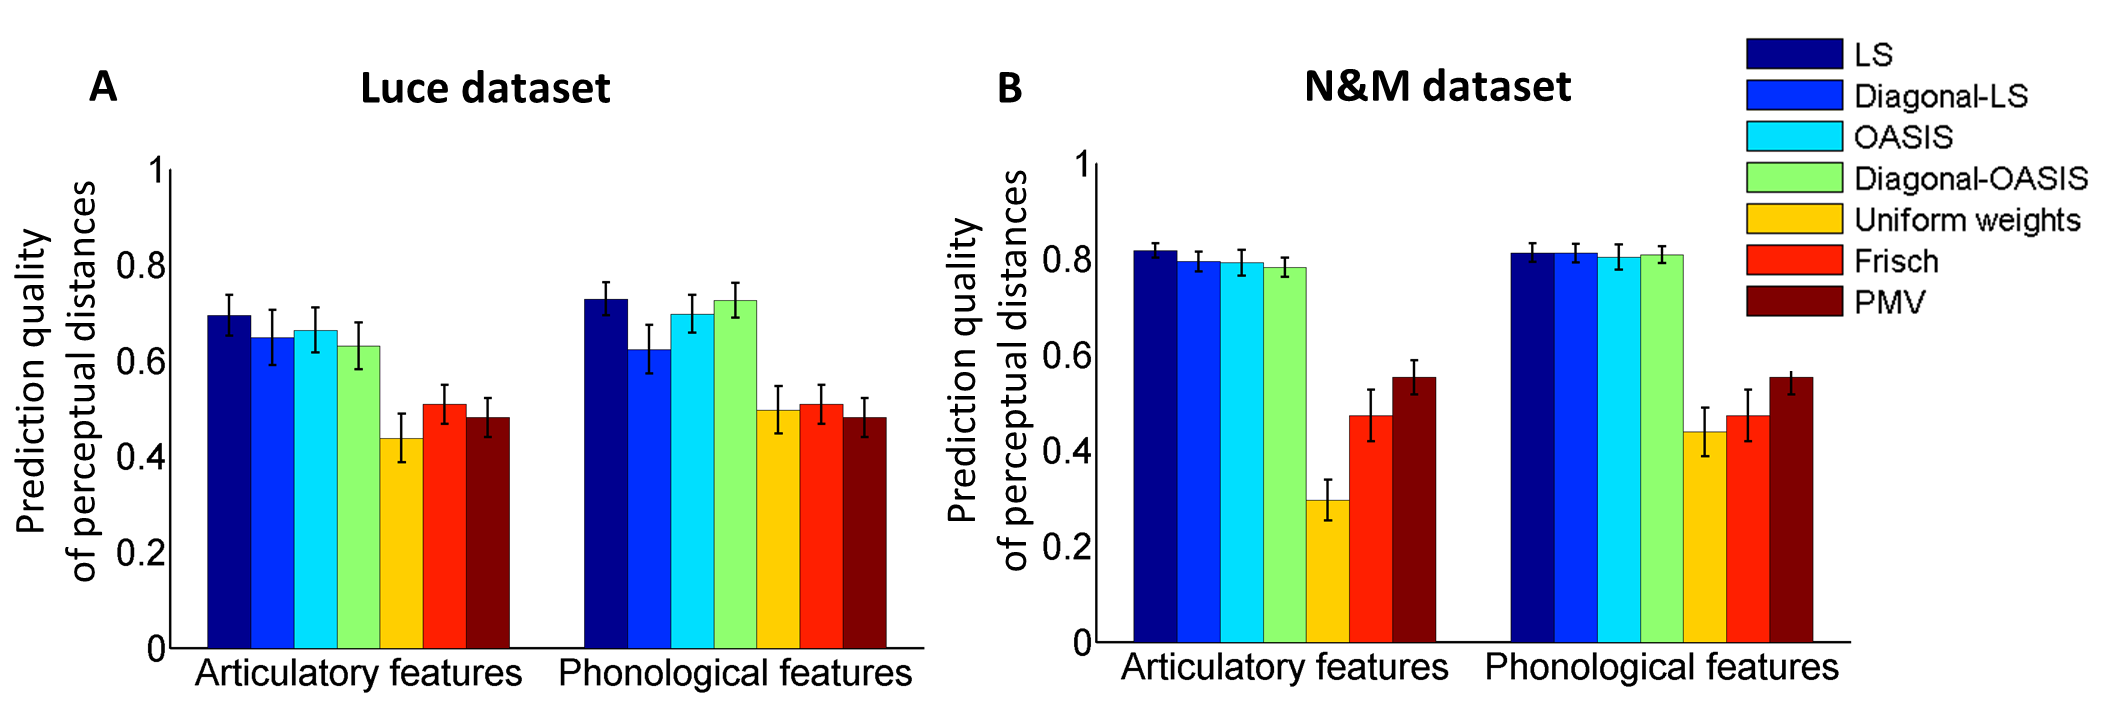
\includegraphics[width=\textwidth]{Figures/Ch2/method_comparison.png}}
\caption{Prediction quality of perceptual distances. For each of the seven methods, the Spearman correlation between the predicted and empirical perceptual distances is calculated, averaged across left-out sets. Error bars represent SD across left-out sets.} 
\end{figure*}

Figure C.8 compares the average Spearman correlation between seven methods. Results are shown for both confusion datasets: N\&M dataset, Luce dataset; and for the two feature theories discussed above: articulatory features and phonological features. Model prediction is evaluated in a cross-validation procedure (methods 2.4). The prediction of the model is defined as the average Spearman correlation across all validation sets, and the standard deviation is evaluated from the distributions across these sets. To determine the optimal regularizer size model predictions are evaluated on a validation set for various values of the regularization.

Figure C.8 shows that learning feature weights from data significantly improves prediction in comparison to baseline methods (For the N\&M dataset, all comparisons between the data-driven methods and the theoretical measures (Frisch, PMV, uniform weighing) have $p$-value$<10^{-4}$ (t-test). For the Luce dataset, Table A.2 summarizes $p$-values).

Results show that all four metric-learning methods demonstrate similar predictive power, as tested on these datasets. We therefore select a method for further analysis based on model parsimony and running time. Adding a diagonal constraint results in a more parsimonious model due to its smaller number of free parameters. Moreover, it is easier to interpret results when the off-diagonal values of the weight matrix are all zero, i.e., without rotations of the feature space. We therefore choose to use diagonal-LS for the analyses in the rest of this study.